\documentclass[11pt]{article}
\usepackage[margin=1in]{geometry}
\usepackage[T1]{fontenc}
\usepackage{lmodern}
\usepackage{amsmath,amssymb,amsthm}
\usepackage{graphicx}
\usepackage[hidelinks]{hyperref}
\usepackage{microtype}
\raggedright

\newtheorem*{theorem}{Theorem}
\newtheorem*{corollary}{Corollary}

\begin{document}

\begin{center}
{\Large Literature-implied full answer for arXiv:1212.6243}\\[4pt]
{\large Dedekind completeness makes Archimedeanness automatic}
\end{center}

\paragraph{Status.}
\textbf{literature\_implied\_answer (full answer to the local question).}
The answer is an immediate consequence of a standard implication in vector
lattice theory.  The contribution of this packet is to notice that the
source's hypotheses already contain that implication, not to claim a new
order-theoretic theorem.

\paragraph{Exact source question.}
Rutsky's Proposition~18 assumes that $Y$ is an \emph{Archimedean Dedekind
complete lattice}. Immediately after its proof, the paper asks whether the
Archimedean assumption is necessary for the conclusion:

\begin{center}
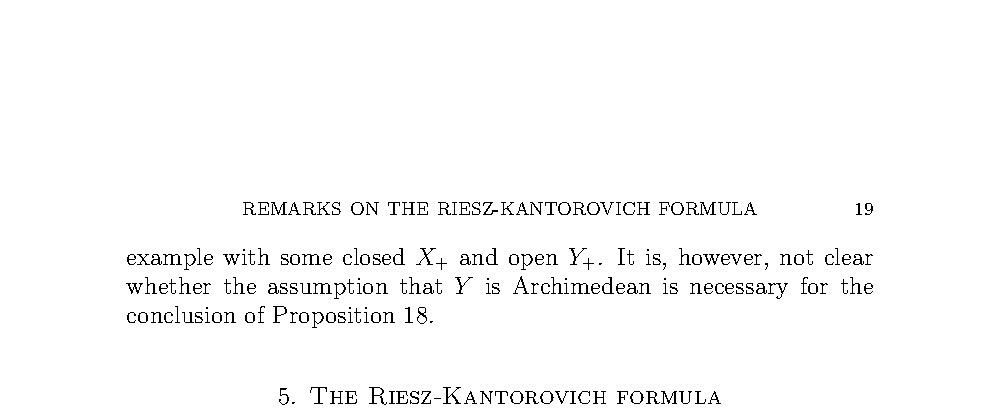
\includegraphics[width=.94\linewidth]{figures/source_question.jpg}
\end{center}

The same paper defines Dedekind completeness to mean that every
upper-bounded subset has a supremum.

\begin{theorem}
Every Dedekind complete real vector lattice $Y$ is Archimedean.  Thus the
answer to the source question is \emph{no}: Archimedeanness is redundant under
the remaining hypotheses of Proposition~18.
\end{theorem}

\begin{proof}
Use exactly the source's definition of Archimedeanness.  Suppose $x\in Y_+$
and $y\in Y$ satisfy
\[
 n y\le x\qquad(n=1,2,\ldots).
\]
The positive-part map of a vector lattice is order preserving, and it is
positively homogeneous.  Hence
\[
 n y^+=(ny)^+\le x^+ = x \qquad(n\ge1).
\]
The set $A=\{ny^+:n\ge1\}$ is therefore bounded above, so Dedekind
completeness gives $s=\sup A$.  Since $y^+\ge0$, this sequence is increasing,
and its tail has the same supremum:
\[
 s=\sup_{n\ge1}(n+1)y^+.
\]
Translation by $y^+$ is an order isomorphism, so it preserves every existing
supremum. Consequently
\[
 s=\sup_{n\ge1}\bigl(y^++ny^+\bigr)
  =y^++\sup_{n\ge1}ny^+=y^++s.
\]
Cancellation yields $y^+=0$, whence $y\le0$.  This is precisely the
Archimedean condition stated immediately before Proposition~18.
\end{proof}

\begin{corollary}
In Proposition~18 of arXiv:1212.6243, delete the word
``Archimedean'' from ``Archimedean Dedekind complete lattice.''  The statement
and proof remain valid.  Likewise, in case~(2) of Theorem~24, the separate
condition that $Y$ be Archimedean may be deleted because the theorem already
assumes globally that $Y$ is a Dedekind complete lattice.
\end{corollary}

\begin{proof}
Apply the theorem to $Y$, then invoke the original results unchanged.
\end{proof}

\paragraph{Why this is literature-implied.}
The implication proved above is standard.  For example, modern vector-lattice
references routinely state that every Dedekind complete vector lattice is
Archimedean.  No additional Riesz--Kantorovich argument is needed.

\paragraph{Relation to the headline problem.}
The introduction also recalls the long-standing question whether an existing
operator supremum must equal its Riesz--Kantorovich transform.  That is a
different question, and this run already has a packet recording Elliott's
2019 negative answer under target arXiv:1501.01685.  The present packet avoids
double-counting that result and promotes only the distinct local question
following Proposition~18.

\paragraph{Verification and search.}
The proof is symbolic and its five order-theoretic steps are audited in
\texttt{verification.md}.  Cheap run indexes were searched for the arXiv id,
title, ``Riesz--Kantorovich'', ``Dedekind complete'', and ``Archimedean.''  A
bounded exact-phrase/title search found the source and standard statements of
the implication, but no later paper devoted to this local question.

\paragraph{Scope.}
This settles the necessity question only while retaining Dedekind completeness
and the lattice hypothesis.  It does not remove Dedekind completeness, answer
the general operator-supremum problem anew, or address the source's speculative
quasi-interior-point extension.

\begin{thebibliography}{9}
\bibitem{Rutsky}
D. V. Rutsky,
\emph{Remarks on the Riesz--Kantorovich formula},
arXiv:1212.6243 (2012; manuscript dated 2014).

\bibitem{Elliott}
M. Elliott,
\emph{The Riesz--Kantorovich formulae},
Positivity \textbf{23} (2019), 1245--1259.
\end{thebibliography}

\end{document}

